\documentclass[12pt, a4paper]{article}

% --- Pakiety ---
\usepackage[utf8]{inputenc}
\usepackage[T1]{fontenc}
\usepackage[polish]{babel}
\usepackage{geometry}
\usepackage{amsmath}
\usepackage{amssymb}
\usepackage{graphicx}
\usepackage{booktabs}
\usepackage{siunitx}
\usepackage{caption}
\usepackage{subcaption}
\usepackage{float}
\usepackage{hyperref}
\usepackage{xcolor}
\usepackage{array}
\usepackage{multirow}
\usepackage{fancyhdr}

% --- Kropka ---
\captionsetup{labelsep=period}

% --- Marginesy ---
\geometry{
    top=2.5cm,
    bottom=2.5cm,
    left=2.5cm,
    right=2.5cm,
    footskip=2cm
}

% --- Stopka ---
\pagestyle{fancy}
\fancyhf{}
\renewcommand{\headrulewidth}{0pt}
\renewcommand{\footrulewidth}{0.4pt}
\fancyfoot[R]{
\includegraphics[height=0.8cm]{lumon.pdf}}

% --- Konfiguracja siunitx ---
\sisetup{
    output-decimal-marker = {,},
    separate-uncertainty = true
}

% --- Dane raportu ---
\newcommand{\tytul}{Badanie drgań wahadeł sprzężonych}
\newcommand{\codeword}{Coleman}
\newcommand{\nrCwiczenia}{M21}
\newcommand{\autor}{Karol Peszek}
\newcommand{\nrGrupy}{B}
\newcommand{\dataWykonania}{13 maja 2026}

% --- Tytuł dokumentu ---
\title{
    \large I Pracownia Fizyczna \\[0.5em]
    \textbf{Ćwiczenie \nrCwiczenia} \\[0.3em]
    \LARGE \tytul\space''\codeword''
}
\author{
    \autor\\
     Grupa \nrGrupy}
\date{
    Data wykonania pomiarów: \dataWykonania\\
}

% =============================================
\begin{document}
% =============================================

\maketitle
\thispagestyle{empty}
\newpage

% -------------------------------------------
\section{Cel ćwiczenia}
% -------------------------------------------

W niniejszej pracy zbadano drgania układu dwóch jednakowych wahadeł fizycznych sprzężonych sprężyną:
wyznaczono okresy drgań swobodnych, zmierzono okresy obu drgań normalnych
i na ich podstawie obliczono moment sprzęgający $D_s$ sprężyny.
Korzystając z pomiarów okresu dudnień przy sześciu różnych odległościach zaczepienia
sprężyny, zweryfikowano kwadratową zależność $D_s = ks^2$ i wyznaczono stałą sprężystości~$k$.

% -------------------------------------------
\section{Wstęp teoretyczny}
% -------------------------------------------

\subsection{Wahadło fizyczne}

Wahadło fizyczne to dowolne ciało sztywne zdolne do swobodnego obrotu wokół poziomej
osi obrotu nieprzechodzącej przez jego środek masy.
Moment siły grawitacji względem osi obrotu, przy małych wychyleniach $\varphi$
od położenia równowagi, wynosi
\begin{equation}
    N_g = mgl\sin(-\varphi) \approx -mgl\,\varphi = -D\varphi,
    \label{eq:Ng}
\end{equation}
gdzie $m$ jest masą wahadła, $l$ odległością środka masy od osi zawieszenia,
a $D = mgl$ jest \emph{momentem kierującym}. Drugie prawo dynamiki dla ruchu
obrotowego $N = J\ddot{\varphi}$ prowadzi do równania oscylatora harmonicznego
o kołowej częstości drgań własnych
\begin{equation}
    \omega_0 = \sqrt{\frac{D}{J}},
    \label{eq:omega0}
\end{equation}
gdzie $J$ jest momentem bezwładności wahadła względem osi obrotu.
Odpowiedni okres drgań swobodnych wynosi $T_0 = 2\pi/\omega_0$.

Moment bezwładności wahadła użytego w ćwiczeniu składa się z dwóch wkładów.
Dla pręta obracającego się wokół jednego końca:
\begin{equation}
    J_\text{rod} = \tfrac{1}{3}m_r l^2.
    \label{eq:Jpret}
\end{equation}
Krążek (walec) jest zamontowany tak, że oś obrotu wahadła jest równoległa
do jednej z jego średnic, w odległości $s$ od środka masy krążka.
Na mocy twierdzenia Steinera:
\begin{equation}
    J_\text{weight} = m_k\!\left(\frac{d^2}{16} + \frac{h^2}{12}\right) + m_k s^2,
    \label{eq:Jkrazek}
\end{equation}
gdzie $d$ jest średnicą, a $h$ grubością krążka. Całkowity moment bezwładności
wahadła wynosi $J = J_\text{rod} + J_\text{weight}$, a moment kierujący:
\begin{equation}
    D = m_r g \frac{l}{2} + m_k g s.
    \label{eq:D}
\end{equation}

\subsection{Układ wahadeł sprzężonych}

Rozważmy dwa jednakowe wahadła fizyczne połączone sprężyną o stałej sprężystości $k$,
zaczepionych w odległości $s$ od osi obrotu (Rysunek~\ref{fig:schemat}).
Przy wychyleniach $\varphi_a$ i $\varphi_b$ sprężyna rozciąga się o
$\Delta x \approx s(\varphi_a - \varphi_b)$,
wytwarzając moment sprzęgający działający na każde z wahadeł.
Oznaczając $D_s = ks^2$, równania ruchu układu mają postać~\cite{skrypt}:
\begin{equation}
    J\ddot{\varphi}_a = -D\varphi_a - D_s(\varphi_a - \varphi_b), \qquad
    J\ddot{\varphi}_b = -D\varphi_b - D_s(\varphi_b - \varphi_a).
    \label{eq:ruchu}
\end{equation}
Wprowadzając podstawienie $D/J = \omega_0^2$ oraz $D_s/J = K$,
układ~\eqref{eq:ruchu} przyjmuje postać:
\begin{equation}
    \ddot{\varphi}_a + \omega_0^2\varphi_a + K(\varphi_a - \varphi_b) = 0, \qquad
    \ddot{\varphi}_b + \omega_0^2\varphi_b + K(\varphi_b - \varphi_a) = 0.
    \label{eq:ruchu2}
\end{equation}

\begin{figure}[H]
    \centering
    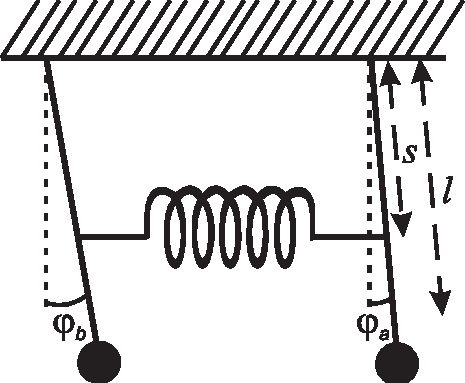
\includegraphics[width=0.45\textwidth]{double_pendulum}
    \caption{Schemat układu dwóch wahadeł sprzężonych sprężyną.
             $s$ --- odległość punktu zaczepienia sprężyny od osi obrotu,
             $\varphi_a$, $\varphi_b$ --- wychylenia wahadeł.
             Źródło:~\cite{skrypt}.}\label{fig:schemat}
\end{figure}

\subsection{Drgania normalne}

Dodając i odejmując równania~\eqref{eq:ruchu2} stronami i wprowadzając
nowe zmienne $\varphi_1 = \tfrac{1}{2}(\varphi_a + \varphi_b)$
oraz $\varphi_2 = \tfrac{1}{2}(\varphi_a - \varphi_b)$, otrzymujemy
dwa niezależne równania oscylatora harmonicznego:
\begin{equation}
    \ddot{\varphi}_1 + \omega_1^2\varphi_1 = 0, \qquad
    \ddot{\varphi}_2 + \omega_2^2\varphi_2 = 0,
    \label{eq:normalne}
\end{equation}
gdzie kołowe częstości drgań normalnych wynoszą odpowiednio:
\begin{equation}
    \omega_1 = \omega_0, \qquad
    \omega_2 = \sqrt{\omega_0^2 + 2K}.
    \label{eq:omega12}
\end{equation}
Pierwsze drganie normalne ($\varphi_1$) odpowiada ruchowi zgodnemu obu wahadeł
z częstością wolną $\omega_1 = \omega_0$ --- sprężyna nie jest rozciągana.
Drugie drganie normalne ($\varphi_2$) odpowiada ruchowi przeciwnemu
z wyższą częstością $\omega_2 > \omega_0$.
Moment sprzęgający wyznacza się wprost z~\eqref{eq:omega12}:
\begin{equation}
    D_s = K \cdot J = \frac{\omega_2^2 - \omega_1^2}{2}\,J.
    \label{eq:Ds_metoda1}
\end{equation}

\subsection{Dudnienia}

Gdy wahadła nie wykonują drgań normalnych, ogólne rozwiązanie dla równych
amplitud i zerowych faz początkowych ma postać:
\begin{align}
    \varphi_a(t) &= 2A\cos\!\left(\tfrac{\omega_2-\omega_1}{2}\,t\right)
                    \cos\!\left(\tfrac{\omega_2+\omega_1}{2}\,t\right), \notag \\
    \varphi_b(t) &= 2A\sin\!\left(\tfrac{\omega_2-\omega_1}{2}\,t\right)
                    \sin\!\left(\tfrac{\omega_2+\omega_1}{2}\,t\right).
    \label{eq:dudnienia}
\end{align}
Każde wahadło drga z częstością nośną $(\omega_2+\omega_1)/2$
i amplitudą modulowaną z częstością dudnień
\begin{equation}
    \omega_d = \omega_2 - \omega_1,
    \label{eq:omegad}
\end{equation}
co zostało zilustrowane na Rysunku~\ref{fig:dudnienia}.
Okres dudnień $T_d = 2\pi/\omega_d$ spełnia związek~\cite{skrypt}:
\begin{equation}
    T_d = \frac{T_0\,T_2}{T_0 - T_2}.
    \label{eq:Td}
\end{equation}
Dla słabego sprzężenia ($K \ll \omega_0^2$), korzystając
z przybliżenia $\sqrt{1+x}\approx 1+\tfrac{1}{2}x$, otrzymujemy:
\begin{equation}
    D_s = 4\pi^2 \frac{J}{T_d\,T_0}.
    \label{eq:Ds_metoda2}
\end{equation}
Ponieważ $D_s = ks^2$, zależność okresu dudnień od odległości
zaczepienia sprężyny ma postać $1/T_d \propto s^2$.

\begin{figure}[H]
    \centering
    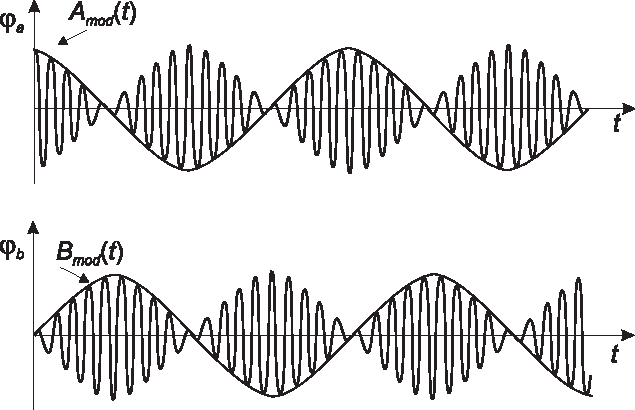
\includegraphics[width=0.72\textwidth]{double_pendulum_waveform}
    \caption{Wychylenia $\varphi_a(t)$ i $\varphi_b(t)$ wahadeł sprzężonych
             wykonujących dudnienia (jednakowe amplitudy drgań normalnych,
             zerowe fazy początkowe). Źródło:~\cite{skrypt}.}\label{fig:dudnienia}
\end{figure}

% -------------------------------------------
\section{Opis układu pomiarowego}
% -------------------------------------------
\begin{figure}[H]
    \centering
    
\includegraphics[width=0.82\textwidth]{schema.jpg}
    \caption{Zdjęcie układu doświadczalnego z wahadłami fizycznymi.}\label{fig:set_photo}
\end{figure}

Do przeprowadzenia pomiarów wykorzystano następujące przyrządy:
\begin{itemize}
    \item dwa jednakowe wahadła fizyczne w postaci prętów zawieszonych na osi obrotu,
    \item dwa krążki (walce) o znanych wymiarach i masie, montowane na prętach,
    \item sprężyna o nieznanej stałej sprężystości mocowana do prętów w odległości $s$ od osi obrotu,
    \item stoper do pomiaru okresów drgań,
    \item suwmiarka o dokładności 0,01 mm do pomiaru wymiarów krążków,
    \item przymiar do pomiaru długości prętów i odległości $s$ z dokładnością 1 mm,
    \item deseczka służąca do jednoczesnego wygaszania obu wahadeł
\end{itemize}

% -------------------------------------------
\section{Procedura pomiarowa}
% -------------------------------------------
W celu zbadania drgań układu wahadeł sprzężonych należy wykonać następujące kroki:
\begin{enumerate}
    \item Zmierzyć średnicę $d$ i grubość $h$ krążków oraz długość $l$ prętów, a także masy $m_r$ prętów i $m_k$ krążków.
    \item Wykonać pomiar 20 okresów drgań swobodnych $T_0$ każdego z wahadeł osobno, bez sprężyny. Pomiar powtórzyć 10 razy dla każdego wahadła.
    \item Zamontować sprężynę między wahadłami.
    \item Wykonać pomiar 20 okresów drgań normalnych $T_1$ (ruch zgodny) i $T_2$ (ruch przeciwny) układu, rozpoczynając od wychylenia obu wahadeł w tym samym kierunku (dla $T_1$) lub w przeciwnych kierunkach (dla $T_2$). Pomiar powtórzyć 3 razy dla każdego rodzaju drgań normalnych.
    \item Dla sześciu różnych odległości $s$ zaczepienia sprężyny, wykonać pomiar 10 okresów dudnień $T_d$ układu, rozpoczynając od wychylenia jednego z wahadeł. Pomiar powtórzyć 3 razy dla każdej odległości $s$.
\end{enumerate}
% -------------------------------------------
\section{Wyniki pomiarów}
% -------------------------------------------

\subsection{Właściwości fizyczne wahadeł}

Zmierzono wymiary geometryczne i masy elementów składowych obu wahadeł.
Wyniki zestawiono w Tabeli~\ref{tab:wymiary}.

\begin{table}[H]
    \centering
    \caption{Wymiary i masy elementów wahadeł.}\label{tab:wymiary}
    \begin{tabular}{lcccc}
        \toprule
        Wielkość & Symbol & Wahadło lewe & Wahadło prawe & Jedn. \\
        \midrule
        Długość pręta           & $l$     & 1150      & 1150      & mm \\
        Masa pręta              & $m_r$   & 834{,}9   & 834{,}9   & g  \\
        Średnica krążka         & $d$     & $95{,}9 \pm 0{,}1$ & $95{,}7 \pm 0{,}1$ & mm \\
        Grubość krążka          & $h$     & $19{,}9 \pm 0{,}1$ & $19{,}9 \pm 0{,}1$ & mm \\
        Masa krążka             & $m_k$   & 1164{,}5  & 1168{,}0  & g  \\
        Odległość krążka od osi & $s_k$   & \multicolumn{2}{c}{$1010 \pm 10$} & mm \\
        Odległość zaczepienia sprężyny & $s$ & \multicolumn{2}{c}{$585 \pm 10$} & mm \\
        \bottomrule
    \end{tabular}
\end{table}

\subsection{Drgania swobodne}

Dla każdego wahadła wykonano 10 pomiarów czasu 20 okresów drgań swobodnych $T_{20}$;
niepewność pojedynczego pomiaru $u(T_{20}) = 0{,}8$~s.
Wyniki zestawiono w Tabeli~\ref{tab:drgania_swobodne}.

\begin{table}[H]
    \centering
    \caption{Czasy 20 okresów drgań swobodnych obu wahadeł.}\label{tab:drgania_swobodne}
    \begin{tabular}{ccc}
        \toprule
        Pomiar & $T_{20}^\text{lewe}$ [s] & $T_{20}^\text{prawe}$ [s] \\
        \midrule
        1  & 39{,}32 & 39{,}61 \\
        2  & 39{,}33 & 39{,}14 \\
        3  & 39{,}40 & 39{,}33 \\
        4  & 39{,}40 & 39{,}47 \\
        5  & 39{,}50 & 39{,}32 \\
        6  & 39{,}46 & 39{,}26 \\
        7  & 39{,}47 & 39{,}51 \\
        8  & 39{,}43 & 39{,}50 \\
        9  & 39{,}29 & 39{,}57 \\
        10 & 39{,}29 & 39{,}29 \\
        \bottomrule
    \end{tabular}
\end{table}

\begin{figure}[H]
    \centering
    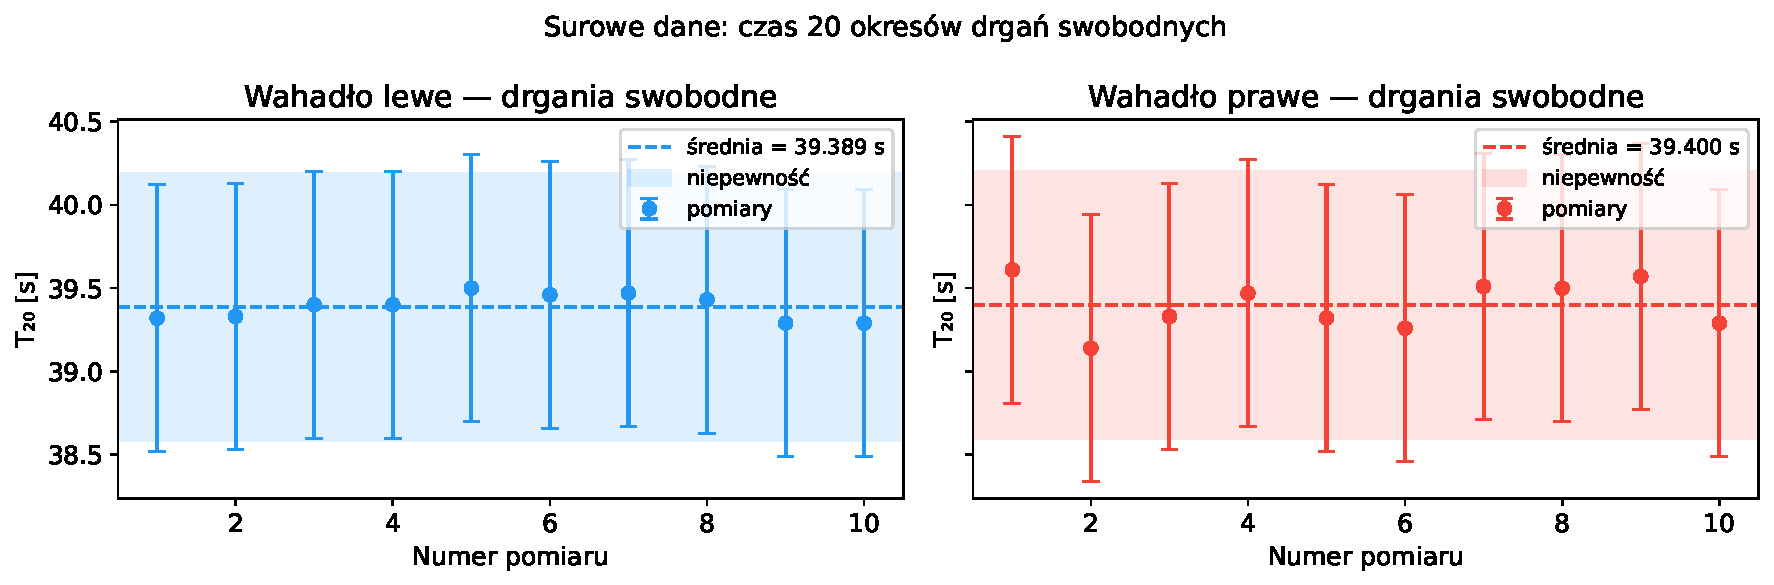
\includegraphics[width=0.75\textwidth]{rys_1_drgania_swobodne_surowe}
    \caption{Czasy 20 okresów drgań swobodnych obu wahadeł --- surowe dane pomiarowe
             z niepewnościami.}\label{fig:drgania_swobodne_surowe}
\end{figure}

\subsection{Drgania normalne}

Przy odległości zaczepienia sprężyny $s = (585 \pm 10)$~mm wykonano po trzy pomiary
czasu 20 okresów każdego z drgań normalnych (Tabela~\ref{tab:drgania_normalne}).

\begin{table}[H]
    \centering
    \caption{Czasy 20 okresów drgań normalnych przy $s = 585$~mm.}\label{tab:drgania_normalne}
    \begin{tabular}{ccc}
        \toprule
        Pomiar & $T_{20}^{(1)}$ [s] & $T_{20}^{(2)}$ [s] \\
        \midrule
        1 & 39{,}01 & 31{,}76 \\
        2 & 38{,}85 & 31{,}66 \\
        3 & 38{,}74 & 31{,}86 \\
        \bottomrule
    \end{tabular}
\end{table}

\begin{figure}[H]
    \centering
    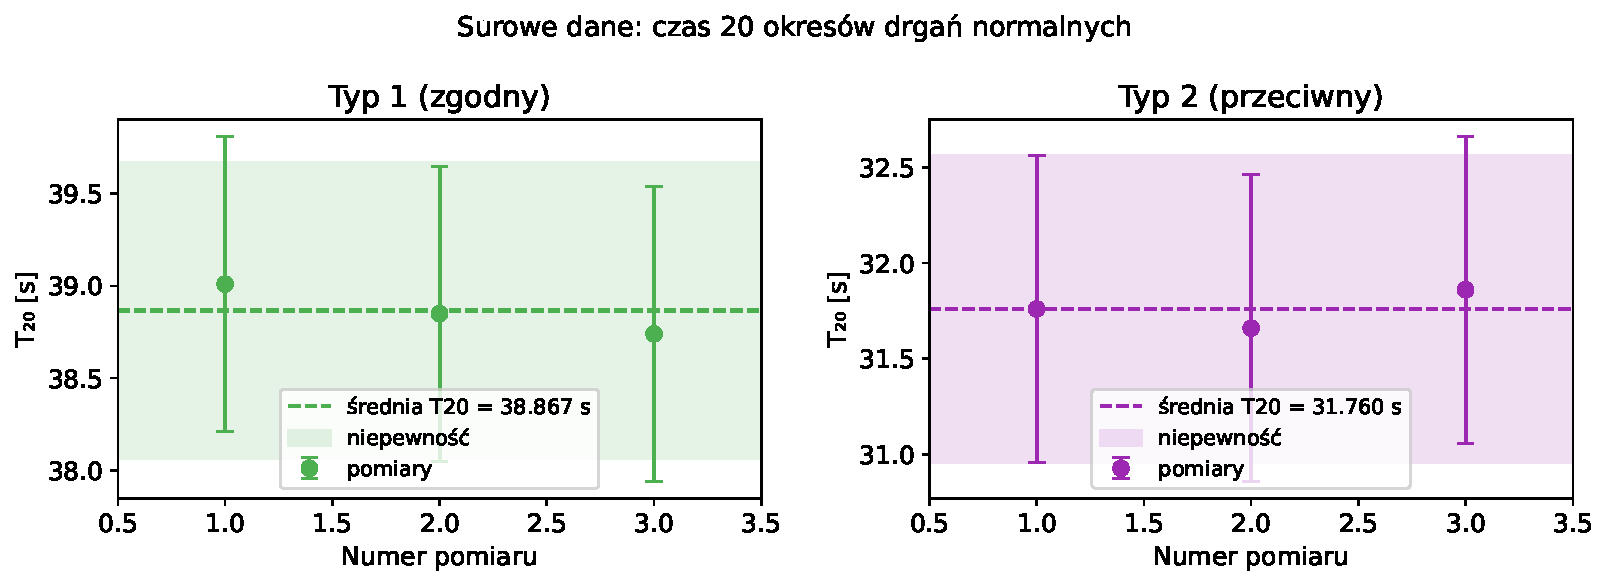
\includegraphics[width=0.75\textwidth]{rys_3_drgania_normalne_surowe}
    \caption{Czasy 20 okresów obu drgań normalnych przy $s = 585$~mm ---
             surowe dane pomiarowe z niepewnościami.}\label{fig:drgania_normalne_surowe}
\end{figure}

\subsection{Dudnienia}

Dla sześciu różnych odległości zaczepienia sprężyny wykonano po trzy pomiary
czasu 10 okresów dudnień $T_{10}$; niepewność pojedynczego pomiaru $u(T_{10}) = 0{,}8$~s.
Wyniki zestawiono w Tabeli~\ref{tab:dudnienia}.

\begin{table}[H]
    \centering
    \caption{Czasy 10 okresów dudnień dla różnych odległości zaczepienia sprężyny.}\label{tab:dudnienia}
    \begin{tabular}{cccc}
        \toprule
        $s$ [mm] & $T_{10}^{(1)}$ [s] & $T_{10}^{(2)}$ [s] & $T_{10}^{(3)}$ [s] \\
        \midrule
        $400 \pm 10$ & 185{,}47 & 187{,}80 & 186{,}62 \\
        $500 \pm 10$ & 119{,}12 & 119{,}56 & 119{,}19 \\
        $600 \pm 10$ &  83{,}02 &  81{,}77 &  81{,}96 \\
        $700 \pm 10$ &  61{,}10 &  60{,}42 &  60{,}51 \\
        $800 \pm 10$ &  47{,}03 &  47{,}37 &  47{,}16 \\
        $900 \pm 10$ &  39{,}52 &  38{,}90 &  38{,}74 \\
        \bottomrule
    \end{tabular}
\end{table}

\begin{figure}[H]
    \centering
    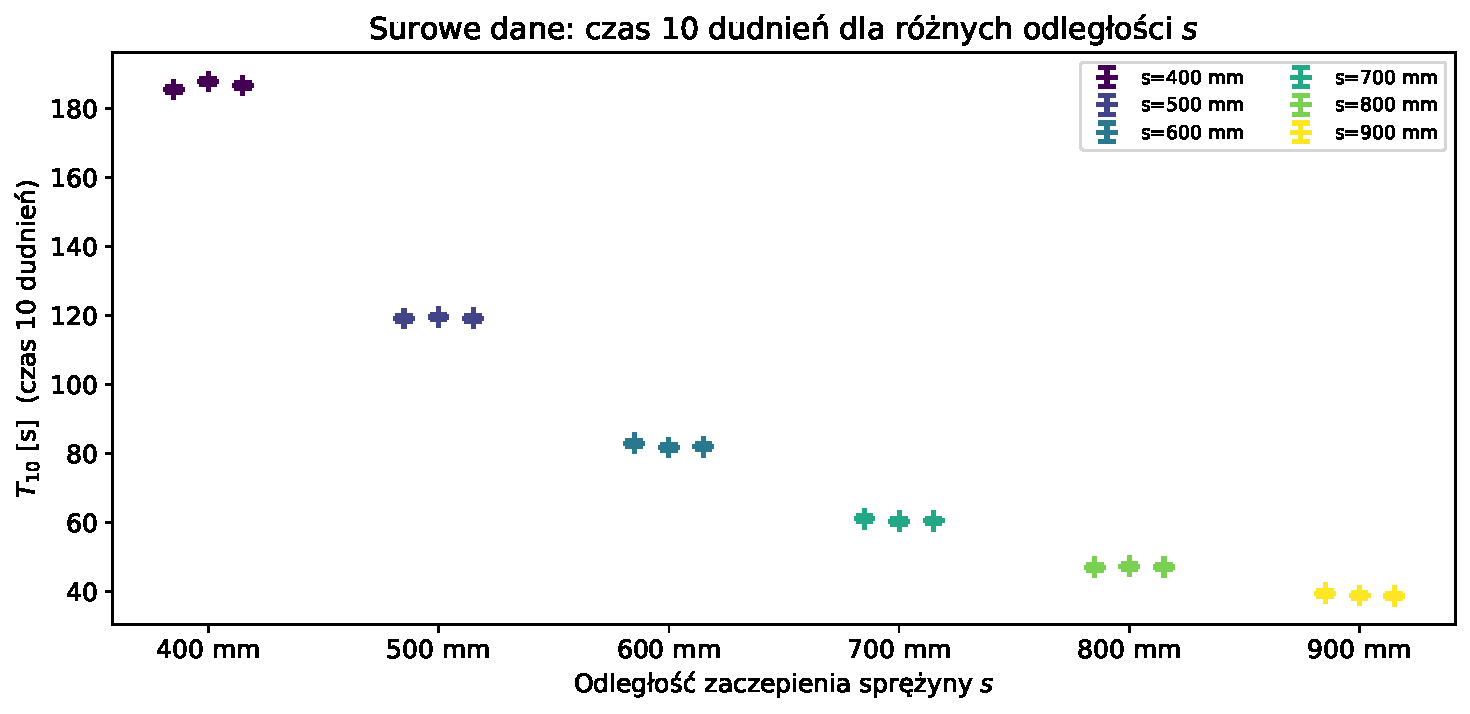
\includegraphics[width=0.75\textwidth]{rys_4_dudnienia_surowe}
    \caption{Czasy 10 okresów dudnień dla różnych odległości zaczepienia sprężyny
             --- surowe dane pomiarowe z niepewnościami.}\label{fig:dudnienia_surowe}
\end{figure}

% -------------------------------------------
\section{Opracowanie wyników}
% -------------------------------------------

\subsection{Moment bezwładności i moment kierujący}

Całkowity moment bezwładności każdego wahadła obliczono ze wzorów~\eqref{eq:Jpret}--\eqref{eq:D}.
Odległość środka masy krążka od osi obrotu wynosi $s_k = (1010\pm10)$~mm.
Niepewność $J_\text{weight}$ wyznaczono metodą propagacji:
\begin{equation}
    u(J_\text{weight}) = m_k\sqrt{{\left(\frac{d}{8}\,u_d\right)}^{\!2}
        + {\left(\frac{h}{6}\,u_h\right)}^{\!2}
        + {(2s_k\,u_{s_k})}^2},
    \label{eq:uJkrazek}
\end{equation}
a moment kierujący: $u(D) = m_k g\,u_{s_k}$.
Ponieważ masy i długość pręta zanotowano bezpośrednio z etykiet,
$u(J_\text{rod}) = 0$ i $u(J) = u(J_\text{weight})$.
Wyniki zestawiono w Tabeli~\ref{tab:JD}.

\begin{table}[H]
    \centering
    \caption{Obliczone momenty bezwładności i kierujące obu wahadeł.}\label{tab:JD}
    \begin{tabular}{lcc}
        \toprule
        Wielkość & Wahadło lewe & Wahadło prawe \\
        \midrule
        $J_\text{weight}$ [$10^{-4}$\,kg\,m$^2$]
            & $11886{,}1\pm235{,}2$ & $11921{,}8\pm235{,}9$ \\
        $J_\text{rod}$ [$10^{-4}$\,kg\,m$^2$]
            & $3680{,}5$ & $3680{,}5$ \\
        $J$ [$10^{-4}$\,kg\,m$^2$]
            & $15566{,}7\pm235{,}2$ & $15602{,}4\pm235{,}9$ \\
        $D$ [N\,m]
            & $16{,}247\pm0{,}114$ & $16{,}282\pm0{,}115$ \\
        $T_{0,\text{teor}}$ [s]
            & $1{,}9448\pm0{,}0162$ & $1{,}9450\pm0{,}0162$ \\
        \bottomrule
    \end{tabular}
\end{table}

Do dalszych obliczeń użyto wartości uśrednionych:
$J_\text{śr} = (1{,}5585\pm0{,}0236)$\,kg\,m$^2$
oraz $D_\text{śr} = (16{,}265\pm0{,}114)$\,N\,m.
Niepewności uśrednionych wartości przyjęto jako niepewności pojedynczego wahadła,
nie redukując ich przez $\sqrt{2}$.
Uzasadnienie: główne źródła niepewności --- pomiar odległości $s_k$ tym samym
przymiarkiem oraz wymiarów $d$, $h$ tym samym śrubomierzem --- są wspólne
dla obu wahadeł, a więc \emph{w pełni skorelowane}.
Dla w pełni skorelowanych błędów systematycznych uśrednienie nie redukuje
niepewności, lecz jedynie przenosi ją na wartość średnią bez zmian.

\subsection{Drgania swobodne}

Okres drgań swobodnych wyznaczono z $N=10$ pomiarów czasu 20 okresów.
Niepewność łączona pojedynczego pomiaru $T_{20}$:
\begin{equation}
    u(T_{20}) = \sqrt{u_A^2 + u_B^2},\qquad
    u_A = \frac{s(T_{20})}{\sqrt{N}},\qquad
    u_B = 0{,}8\text{ s},
    \label{eq:uT20}
\end{equation}
a okres: $T_0 = \langle T_{20}\rangle/20$, $u(T_0) = u(T_{20})/20$.
Uzyskano:
\begin{equation}
    T_0^\text{lewe}  = (1{,}96945\pm0{,}04002)\text{ s},\qquad
    T_0^\text{prawe} = (1{,}97000\pm0{,}04007)\text{ s}.
\end{equation}
Różnica $|T_0^\text{lewe} - T_0^\text{prawe}| = 5{,}5\times10^{-4}$~s
jest znacznie mniejsza niż niepewność różnicy $u_{\Delta T} = 566\times10^{-4}$~s,
zatem wahadła można uznać za identyczne.
Uśredniony okres i częstość doświadczalna:
\begin{equation}
    T_{0,\text{exp}} = (1{,}96972\pm0{,}02832)\text{ s},\qquad
    \omega_{0,\text{exp}} = (3{,}1899\pm0{,}0459)\text{ rad/s}.
\end{equation}
Porównanie z wartościami teoretycznymi (Rysunek~\ref{fig:T0_compare})
pokazuje zgodność w granicach niepewności.

\begin{figure}[H]
    \centering
    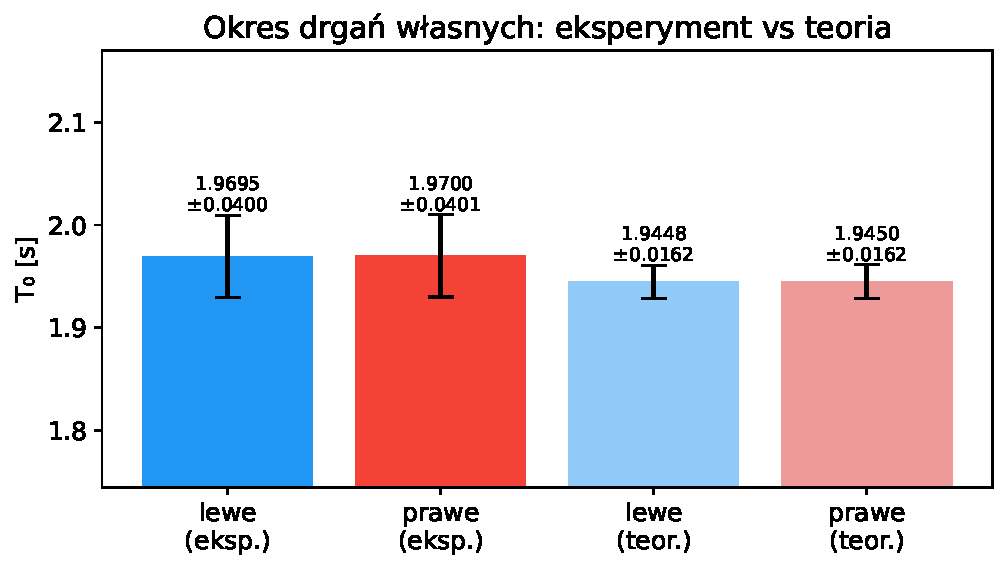
\includegraphics[width=0.72\textwidth]{rys_2_T0_eksp_vs_teoria}
    \caption{Porównanie zmierzonych i obliczonych teoretycznie
             okresów drgań swobodnych obu wahadeł.}\label{fig:T0_compare}
\end{figure}

\subsection{Drgania normalne --- wyznaczenie \texorpdfstring{$D_s$}{Ds} metodą 1}

Okresy drgań normalnych wyznaczono z $N=3$ pomiarów $T_{20}$ przy $s=585$~mm,
stosując wzór~\eqref{eq:uT20}:
\begin{equation}
    T_1 = (1{,}9433\pm0{,}0402)\text{ s},\qquad
    \omega_1 = (3{,}2332\pm0{,}0669)\text{ rad/s},
\end{equation}
\begin{equation}
    T_2 = (1{,}5880\pm0{,}0401)\text{ s},\qquad
    \omega_2 = (3{,}9567\pm0{,}0999)\text{ rad/s}.
\end{equation}
Zgodnie z teorią pierwsze drganie normalne ma częstość $\omega_1 = \omega_0$,
wyznaczaną niezależnie z wymiarów i mas wahadła ze wzoru~\eqref{eq:omega0}:
\begin{equation}
    \omega_{0,\text{teor}} = \sqrt{\frac{D_\text{śr}}{J_\text{śr}}}
                           = (3{,}2306\pm0{,}0269)\text{ rad/s}.
\end{equation}
Porównanie z wartością zmierzoną:
\begin{equation}
    \omega_1 = (3{,}2332\pm0{,}0669)\text{ rad/s}, \qquad
    |\omega_1 - \omega_{0,\text{teor}}| = 0{,}003\text{ rad/s},
\end{equation}
przy niepewności łączonej $u = 0{,}072$~rad/s, co daje zgodność
w granicach $0{,}04\,\sigma$ --- wynik w pełni potwierdzający teorię.
Moment sprzęgający ze wzoru~\eqref{eq:Ds_metoda1}:
\begin{equation}
    D_s^{(1)} = \frac{\omega_2^2-\omega_1^2}{2}\,J_\text{śr}
              = (4{,}053\pm0{,}705)\text{ N\,m}.
    \label{eq:Ds1_wynik}
\end{equation}
Niepewność wyznaczono ze standardowej propagacji niepewności
wzoru~\eqref{eq:Ds_metoda1} przy $s=585$~mm.

\subsection{Dudnienia --- weryfikacja \texorpdfstring{$D_s \propto s^2$}{Ds proportional to s\texttwosuperior} i wyznaczenie \texorpdfstring{$k$}{k}}

Dla każdej odległości $s$ obliczono okres dudnień $T_d = \langle T_{10}\rangle/10$
i moment sprzęgający z przybliżonego wzoru~\eqref{eq:Ds_metoda2}, używając
$T_{0,\text{exp}}$ i $J_\text{śr}$:
\begin{equation}
    \frac{u(D_s)}{D_s} = \sqrt{{\left(\frac{u_{T_d}}{T_d}\right)}^{\!2}
        + {\left(\frac{u_{T_0}}{T_0}\right)}^{\!2}
        + {\left(\frac{u_J}{J}\right)}^{\!2}}.
\end{equation}
Wyniki zestawiono w Tabeli~\ref{tab:dudnienia_wyniki}.

\begin{table}[H]
    \centering
    \caption{Okresy dudnień, kołowe częstości i momenty sprzęgające
             dla różnych odległości zaczepienia sprężyny.}\label{tab:dudnienia_wyniki}
    \begin{tabular}{cccccc}
        \toprule
        $s$ [mm] & $T_d$ [s] & $u(T_d)$ [s] &
        $\omega_d$ [rad/s] & $D_s$ [N\,m] & $u(D_s)$ [N\,m] \\
        \midrule
        400 & 18{,}663 & 0{,}105 & 0{,}337 & 1{,}674 & 0{,}036 \\
        500 & 11{,}929 & 0{,}081 & 0{,}527 & 2{,}618 & 0{,}057 \\
        600 &  8{,}225 & 0{,}089 & 0{,}764 & 3{,}798 & 0{,}089 \\
        700 &  6{,}068 & 0{,}083 & 1{,}036 & 5{,}148 & 0{,}128 \\
        800 &  4{,}719 & 0{,}081 & 1{,}332 & 6{,}620 & 0{,}178 \\
        900 &  3{,}905 & 0{,}083 & 1{,}609 & 7{,}998 & 0{,}239 \\
        \bottomrule
    \end{tabular}
\end{table}

Liniowe dopasowanie $1/T_d = a\,s^2$ do danych ważonych niepewnościami
(Rysunek~\ref{fig:kwadratowa}) potwierdza kwadratową zależność:
\begin{equation}
    a = (0{,}33464\pm0{,}00124)\text{ s}^{-1}\text{m}^{-2}.
\end{equation}
Dopasowanie modelu $D_s = ks^2$ (Rysunek~\ref{fig:Ds_fit}) daje stałą sprężystości:
\begin{equation}
    k = (10{,}40\pm0{,}10)\text{ N/m}.
    \label{eq:k_wynik}
\end{equation}

\begin{figure}[H]
    \centering
    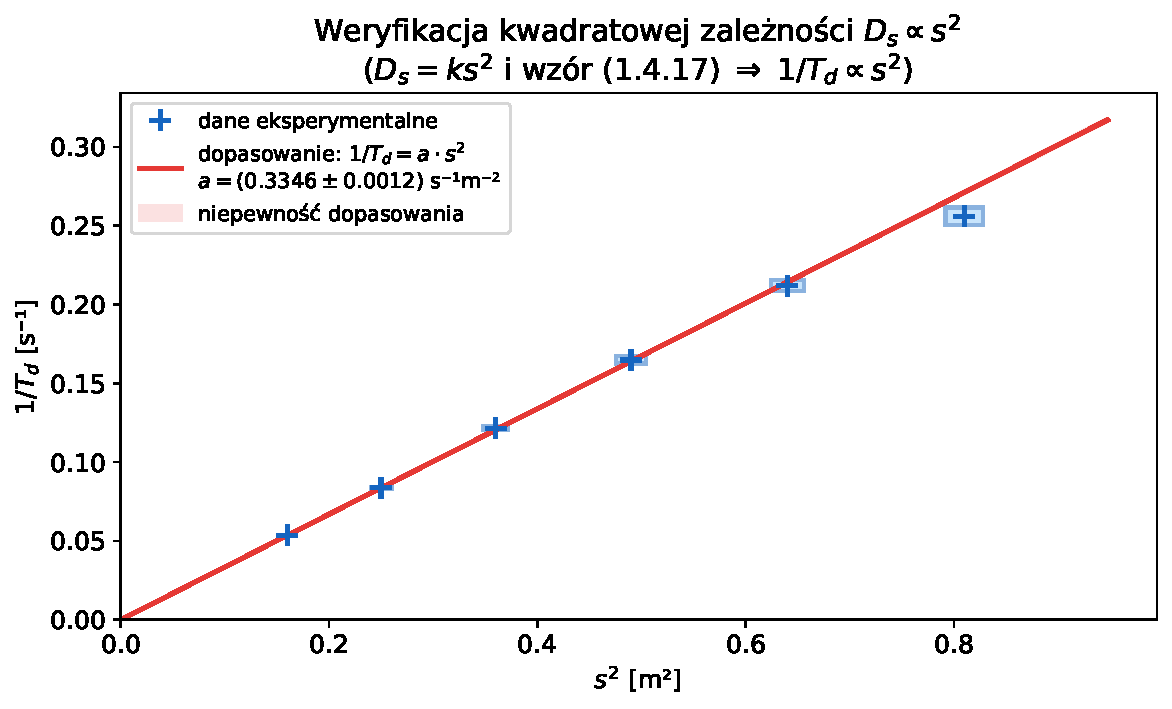
\includegraphics[width=0.72\textwidth]{rys_5a_kwadratowa_zaleznosc}
    \caption{Weryfikacja kwadratowej zależności $D_s\propto s^2$:
             zależność $1/T_d$ od $s^2$ z liniowym dopasowaniem przez początek układu.}\label{fig:kwadratowa}
\end{figure}

\begin{figure}[H]
    \centering
    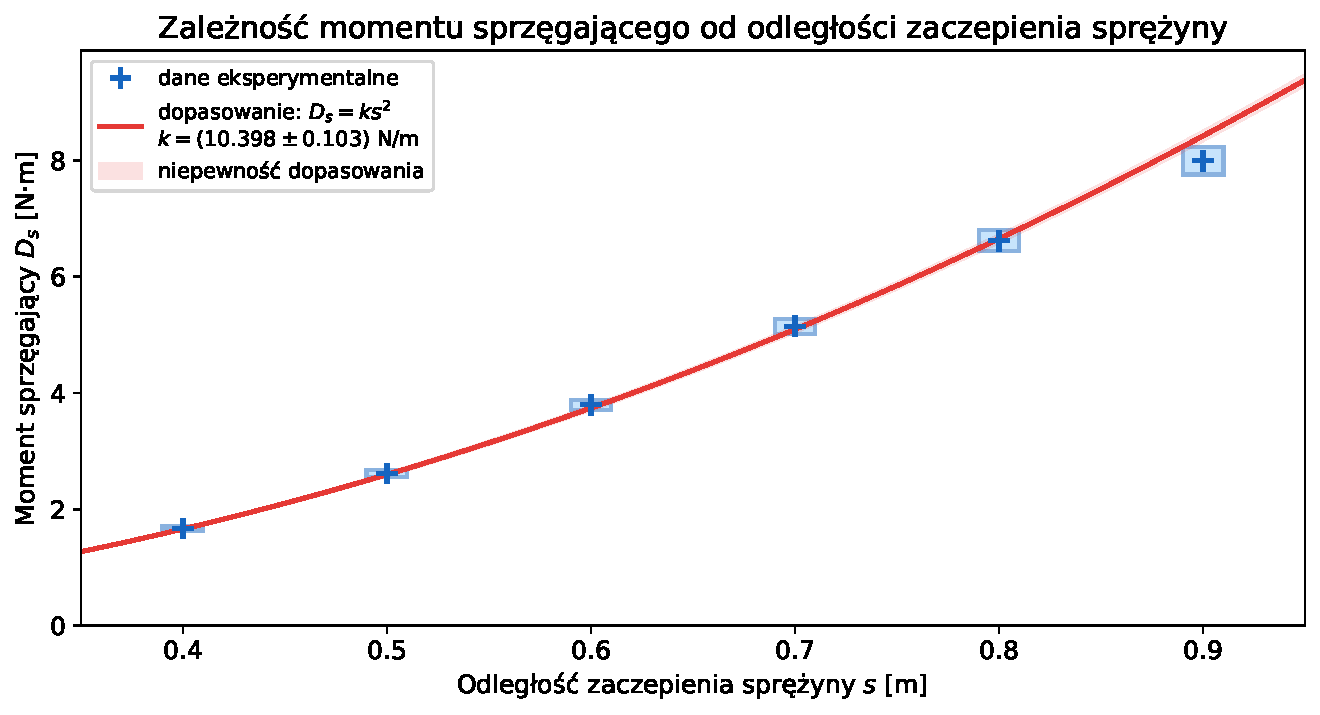
\includegraphics[width=0.72\textwidth]{rys_5b_Ds_dopasowanie}
    \caption{Moment sprzęgający $D_s$ w funkcji odległości zaczepienia sprężyny $s$
             z dopasowaniem modelu $D_s = ks^2$.}\label{fig:Ds_fit}
\end{figure}

Z dopasowania przy $s = 585$~mm, propagując niepewności $u(k)$ i $u(s)$:
\begin{equation}
    u(D_s^{(2)}) = \sqrt{{(s^2\,u_k)}^2 + {(2ks\,u_s)}^2}
                 = \sqrt{0{,}035^2 + 0{,}122^2} \approx 0{,}127\text{ N\,m},
\end{equation}
\begin{equation}
    D_s^{(2)} = k\,s^2 = (3{,}558\pm0{,}127)\text{ N\,m}.
    \label{eq:Ds2_wynik}
\end{equation}
Wkład od $u(s)$ jest tu dominujący.

\subsection{Weryfikacja wzoru (1.4.16)}

Wzór~\eqref{eq:Td} wymaga okresu drgań swobodnych $T_0$, wyznaczanego niezależnie
od drgań normalnych. Podstawiając $T_{0,\text{exp}} = (1{,}96972\pm0{,}02832)$~s
i $T_2 = (1{,}5880\pm0{,}0401)$~s, otrzymano:
\begin{equation}
    T_d^\text{teor} = \frac{T_{0,\text{exp}}\,T_2}{T_{0,\text{exp}}-T_2}
                    = (8{,}194\pm1{,}175)\text{ s}.
\end{equation}
Wartość doświadczalna z dopasowania $D_s(s)$ przy $s=585$~mm
(obliczona konsekwentnie z $T_{0,\text{exp}}$ i pełnym $u(D_s^{(2)}) = 0{,}127$~N\,m):
$T_d^\text{exp} = (8{,}78\pm0{,}36)$~s.
Różnica $0{,}58$~s mieści się w granicach niepewności łączonej $1{,}23$~s --- wyniki zgodne.

Sprawdzono również wzór~\eqref{eq:omega12}:
\begin{equation}
    \omega_2 = \sqrt{\omega_1^2 + 2K},\qquad K = \frac{D_s^{(2)}}{J_\text{śr}}.
    \label{eq:omega2_check}
\end{equation}
Podstawiając $\omega_1 = (3{,}2332\pm0{,}0669)$~rad/s,
$D_s^{(2)} = (3{,}558\pm0{,}035)$~N\,m i $J_\text{śr} = (1{,}5585\pm0{,}0236)$~kg\,m$^2$
($K = (2{,}283\pm0{,}036)$~rad$^2$/s$^2$), otrzymano
(tu $s$ jest ustalone i nie wnosi niepewności do $K$, stąd $u(D_s) = s^2 u_k = 0{,}035$~N\,m):
\begin{equation}
    \omega_{2,\text{teor}} = (3{,}876\pm0{,}057)\text{ rad/s}.
\end{equation}
Wartość zmierzona $\omega_2 = (3{,}957\pm0{,}100)$~rad/s --- różnica $0{,}081$~rad/s
przy niepewności łączonej $0{,}115$~rad/s, wyniki zgodne w granicach $1\sigma$.

\subsection{Porównanie metod wyznaczania momentu sprzęgającego}

\begin{figure}[H]
    \centering
    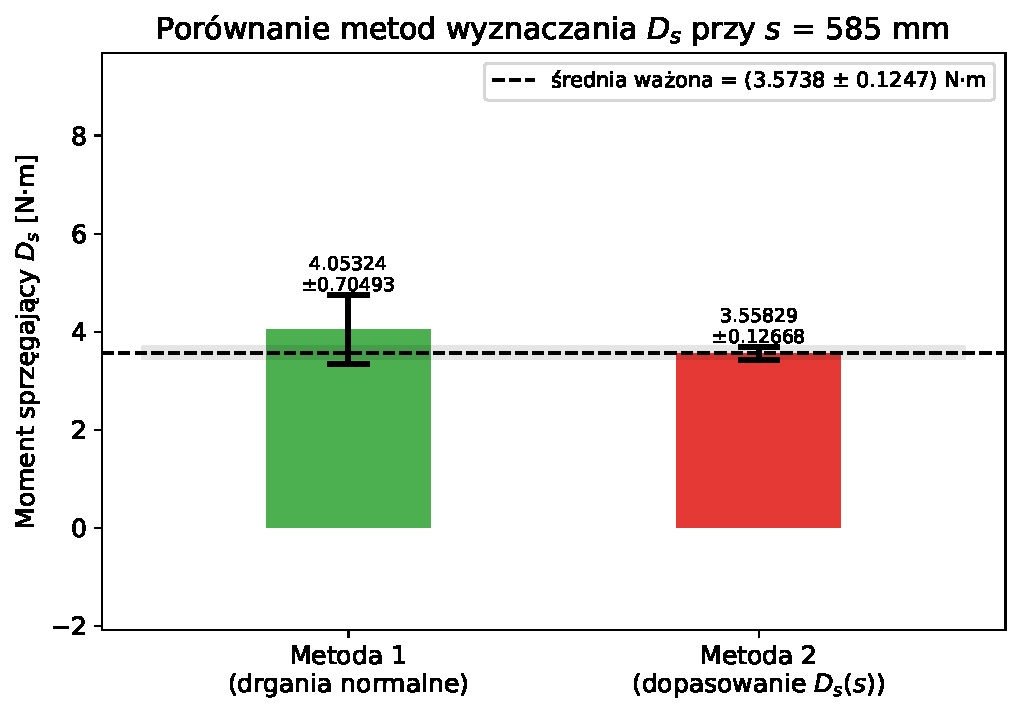
\includegraphics[width=0.65\textwidth]{rys_7_porownanie_Ds}
    \caption{Porównanie momentu sprzęgającego $D_s$ przy $s=585$~mm
             wyznaczonego dwiema metodami.}\label{fig:porownanie_Ds}
\end{figure}

Obie wartości $D_s$~\eqref{eq:Ds1_wynik} i~\eqref{eq:Ds2_wynik} zestawiono
na Rysunku~\ref{fig:porownanie_Ds}. Różnica $0{,}495$~N\,m jest mniejsza niż
niepewność łączona $0{,}718$~N\,m, zatem wyniki są zgodne.
Średnia: $D_s = (3{,}574\pm0{,}125)$~N\,m.

\textbf{Która metoda jest bardziej precyzyjna?}
Metoda~2 (dopasowanie do serii dudnień przy sześciu odległościach $s$) daje
$u(D_s^{(2)}) = 0{,}127$~N\,m, czyli ponad pięciokrotnie mniejszą niepewność
niż metoda~1 ($u(D_s^{(1)}) = 0{,}705$~N\,m).
Przewaga metody~2 wynika z redundancji sześciu punktów pomiarowych,
które przy dopasowaniu modelem $D_s = ks^2$ efektywnie uśredniają błędy
losowe poszczególnych pomiarów okresu dudnień.
W obu metodach dominującym źródłem niepewności jest pomiar odległości
$s$ z niepewnością $u(s) = 10$~mm; w metodzie~1 dochodzi jeszcze duże $u(T_{20})$
przy zaledwie trzech powtórzeniach.

% -------------------------------------------
\section{Wnioski}
% -------------------------------------------

Przeprowadzone ćwiczenie pozwoliło w pełni zrealizować założone cele.
Zmierzone okresy drgań swobodnych obu wahadeł, $T_0^\text{lewe} = (1{,}9695\pm0{,}0400)$~s
i $T_0^\text{prawe} = (1{,}9700\pm0{,}0401)$~s, są zgodne w granicach niepewności,
co potwierdza, że oba wahadła można traktować jako identyczne.
Wartości doświadczalne pozostają ponadto w zgodzie z obliczonymi teoretycznie
na podstawie wymiarów geometrycznych i mas elementów składowych.

Zmierzone okresy drgań normalnych $T_1 = (1{,}9433\pm0{,}0402)$~s
i $T_2 = (1{,}5880\pm0{,}0401)$~s pozwoliły wyznaczyć moment sprzęgający
metodą~1: $D_s^{(1)} = (4{,}053\pm0{,}705)$~N\,m.
Potwierdzona została zgodność częstości $\omega_1$ pierwszego drgania normalnego
z częstością własną $\omega_0$, zgodnie z przewidywaniem teorii.

Z serii pomiarów dudnień dla sześciu różnych odległości zaczepienia sprężyny
potwierdzono kwadratową zależność $D_s \propto s^2$: dopasowanie liniowe
zależności $1/T_d$ od $s^2$ przechodzi przez początek układu współrzędnych,
co jest wyraźnym potwierdzeniem modelu $D_s = ks^2$.
Wyznaczona stała sprężystości sprężyny wynosi $k = (10{,}40\pm0{,}10)$~N/m.
Wartość momentu sprzęgającego uzyskana tą metodą,
$D_s^{(2)} = (3{,}558\pm0{,}127)$~N\,m, jest zgodna z wynikiem metody~1
w granicach niepewności pomiarowych.
Metoda~2 zapewnia większą precyzję ($u = 0{,}127$~N\,m) niż metoda~1
($u = 0{,}705$~N\,m) dzięki redundancji sześciu punktów pomiarowych,
które uśredniają błędy losowe; w obu przypadkach dominującym źródłem
niepewności jest $u(s) = 10$~mm.
Zweryfikowano wzór~\eqref{eq:Td} łączący okresy dudnień i drgań normalnych:
podstawiając $T_{0,\text{exp}}$ z drgań swobodnych, przewidywana wartość
$T_d^\text{teor} = (8{,}19\pm1{,}18)$~s jest zgodna z doświadczalną
$T_d^\text{exp} = (8{,}78\pm0{,}36)$~s.
Potwierdzono ponadto wzór~\eqref{eq:omega12}: częstość $\omega_2$ wyznaczona
z pomiaru czasu drgań normalnych, $\omega_2 = (3{,}957\pm0{,}100)$~rad/s,
jest zgodna z wartością obliczoną ze wzoru $\omega_2 = \sqrt{\omega_1^2 + 2K}$,
wynoszącą $(3{,}876\pm0{,}057)$~rad/s --- różnica mieści się w granicach
pojedynczej niepewności złożonej.

\begin{thebibliography}{9}
\bibitem{skrypt}
\textit{Skrypt do ćwiczeń laboratoryjnych z fizyki, I Pracownia Fizyczna}, ćwiczenie M21.
\end{thebibliography}

\end{document}
% =============================================
